\documentclass{article}

% if you need to pass options to natbib, use, e.g.:
% \PassOptionsToPackage{numbers, compress}{natbib}

% ready for submission
\usepackage{aaai}

% to compile a preprint version, e.g., for submission to arXiv, add
% add the [preprint] option:
% \usepackage[preprint]{nips_2018}

% to compile a camera-ready version, add the [final] option, e.g.:
% \usepackage[final]{nips_2018}

% to avoid loading the natbib package, add option nonatbib:
% \usepackage[nonatbib]{nips_2018}

\usepackage[utf8]{inputenc} % allow utf-8 input
\usepackage[T1]{fontenc}    % use 8-bit T1 fonts
\usepackage{hyperref}       % hyperlinks
\usepackage{url}            % simple URL typesetting
\usepackage{booktabs}       % professional-quality tables
\usepackage{amsfonts}       % blackboard math symbols
\usepackage{nicefrac}       % compact symbols for 1/2, etc.
\usepackage{microtype}      % microtypography
\usepackage{amssymb}
\usepackage{natbib}
%% The amsthm package provides extended theorem environments
\usepackage{amsthm}
\usepackage{float}
\usepackage{sgame, tikz} % Game theory packages
\usepackage{caption} 
\usepackage{algorithm,algpseudocode}
\usepackage{makecell}
 \usepackage{multirow}
 \usepackage{graphicx}
\theoremstyle{definition}
\newtheorem{definition}{Definition}[section]
\captionsetup{font=footnotesize}
\bibliographystyle{aaai}


\title{Competing Bandits}

% The \author macro works with any number of authors. There are two
% commands used to separate the names and addresses of multiple
% authors: \And and \AND.
%
% Using \And between authors leaves it to LaTeX to determine where to
% break the lines. Using \AND forces a line break at that point. So,
% if LaTeX puts 3 of 4 authors names on the first line, and the last
% on the second line, try using \AND instead of \And before the third
% author name.

 \author{-}
  %% Affiliation \\
  %% Address \\
  %% \texttt{email} \\
  %% \And
  %% Coauthor \\
  %% Affiliation \\
  %% Address \\
  %% \texttt{email} \\
  %% \And
  %% Coauthor \\
  %% Affiliation \\
  %% Address \\
  %% \texttt{email} \\

\begin{document}

\maketitle

\begin{abstract}
...
\end{abstract}

\section{Introduction}
\label{S:1}

...

\section{Related Work}
\label{S:2}

\citealt*{mansour2017competing}, \citealt*{che2017recommender}, \citealt*{kremer2014implementing}, \citealt*{mansour2015bayesian}, etc.

\section{Model}
\label{S:3}

...

\section{Simulation Details}
\label{S:4}

\subsection{Bandit Priors}
We study the implications of our model via simulation. For computational tractability we focus our attention on Bernoulli bandits with beta priors. We consider the following bandit ``priors" from which the bandit instances faced in simulation are drawn:
\begin{enumerate}
\item ``HeavyTail": We took the mean rewards to be randomly drawn from Beta($\alpha=0.6,\beta=0.6$). With this distribution it was likely to have arms that were at the extremes (close to 1 and close to 0) but also some of the arms with intermediate value means. [We should rename this prior instance]
\item Needle-in-haystack High - $K-1$ arms with mean 0.50, 1 arm with mean 0.70. 
\end{enumerate}

[Need some discussion of what makes these priors at all ``representative" - why can we just focus on them?]

[We can't feasibly include all the priors. I think Heavy Tail is interesting because of the relative reputation plots, but I'm not sure what other one to include that would be meaningful. For now I've just used NIH]

In the appendix we consider the performance of additional priors, but qualitatively the results presented are unchanged.

\subsection{Learning Algorithms}

For our simulations we evaluate the performance of three algorithms, each endowed with a ``fake prior" of $Beta(1, 1)$. In general, there are three different classes of learning algorithms and we select one representative algorithm from each class: 
\begin{enumerate}
\item Adaptive exploration algorithms that engage in purposeful exploration in a ``smart" way by adapting to the previous history of results. We consider $Thompson Sampling$ (from hereon $TS$) from this class, which, in a given period, will pull an arm according to the probability that that arm is ``optimal" in the sense of having the highest mean reward.
\item Non-adaptive exploration algorithms that engage in purposeful exploration without considering the past results. We consider $Dynamic$ $\epsilon$-$greedy$ (from hereon $DEG$) from this class, which, in a given period, pulls the arms with the highest posterior mean for $1 - \epsilon$ probability and selects a random arm with $\epsilon$ probability. For our experiments we keep $\epsilon = 0.05$ fixed.
\item Greedy / Myopic algorithms that engage in no purposeful exploration and take the best short-sighted action. We consider $DynamicGreedy$ (from hereon $DG$) from this class, which, in a given period, pulls the arm with the highest posterior mean.
\end{enumerate}

Run in isolation we expect that the performance of the algorithms (according to cumulative regret) should be \\
 Adaptive Exploration $>=$ Non-adaptive exploration $>=$ Greedy. We verify that, for the chosen algorithms and chosen priors, this is indeed the case (with some caveats, discussed in the next section).

The primary question that we are interested in is under what conditions in competition are the firms in our model incentivized to commit to adaptive exploration algorithms.

\subsection{Simulation of Competition Game}
Algorithm \ref{alg_1} (FIX TO BE FIGURE) describes the simulation procedure utilized to evaluate the results of the competition game. $T$ is the finite time horizon of the competition game and $K$ is the number of arms in the bandit instance that is considered.

\begin{algorithm}
\caption{Simulation Pseudo-Code}
\begin{algorithmic}[1]
\For{Each prior $p$}
\State Generate true distribution from $p$
\State Generate $T \times K$ realizations for the arms 
	\For{Each agent algorithm $agent alg$}
		\For{Each principal algorithm pair $principalalg1$, $principalalg2$}
			\For{$N$ simulations}
				\State Give principal 2 $X$ free observations (the agents also get these observations)				
				\State Give the agents $k$ observations from each principal (warm start)
				\State Run simulation for $T$ periods
			\EndFor
		\EndFor
	\EndFor
\EndFor
\end{algorithmic}
\label{alg_1}
\end{algorithm}

\section{Performance in Isolation}
\label{S:5}

We look at the performance of each of our learning algorithms in isolation, meaning that we simply run the learning algorithm for $T$ steps on a realization of the prior instances that we consider and record the realized rewards and the arm that is pulled. In our simulations the realizations of each of the arms were pre-drawn and the same across all algorithms and so the differences in algorithm performance come from the difference in the arms selected by the algorithms and not from differences in realizations. When looking at the results of each of the learning algorithms in isolation we want to confirm that, for the prior instances that we consider, ``better" algorithms win according to ``absolute" measures of performance (i.e. looking at mean reputation). Additionally, we want to understand what statistics we can look at in isolation to understand what wins under competition.

In our model the reputation score is an input to the decision rule of the agents and thus it is important to understand how this score differs across algorithms when run outside of competition. Figure \ref{prelim_means} displays the mean average reputation score of each of the algorithms across the different simulations.

\begin{figure}
\caption{Reputation Trajectories in Isolation}
\includegraphics[scale=0.2]{"figures/Reputation Trajectory for Heavy Tail 10 arms"}
\includegraphics[scale=0.2]{"figures/Reputation Trajectory for Needle In Haystack High 10 arms"}
\label{prelim_means}
\caption*{\tiny{The plots contain the average reputation over $250$ runs for a memory size of $100$ where, for a given $t$, we record the reputation of a given algorithm on a given instance and then average this value across all the runs. TODO: get rid of smoothing on plot}}
\end{figure}

\begin{figure}
\caption{Relative Reputation Plots}
\includegraphics[scale=0.25]{"figures/deg_dg_ht_10_prelim"}
\includegraphics[scale=0.25]{"figures/ts_dg_ht_10_prelim"} \\
\includegraphics[scale=0.25]{"figures/deg_dg_nih_10_prelim"}
\includegraphics[scale=0.25]{"figures/ts_dg_nih_10_prelim"} \\
\caption*{\tiny{The plots contain the proportion of simulations over $250$ runs for a memory size of $100$ where, for a given $t$, the reputation of one algorithm is at least as high as the reputation of another on the same instance.}}
\label{relative_rep}
\end{figure}

As expected we see that according to the mean reputation plots $TS > DEG > DG$ for sufficiently large values of $t$. While looking at the mean reputation is a natural statistic to consider when attempting to understand what algorithm wins under competition, we consider an additional statistic when attempting to understand what wins under competition. In the competition game the decision rule of the agents compares the relative reputation of the two firms so that if the reputation of firm $A$ is higher than that of firm $B$, the agents will (be more likely to) select firm $A$. Thus, another natural statistic to look at is to look at the two algorithms in isolation and consider the fraction of simulations where, for a fixed time $t$, the reputation of firm $A$ is at least as high as that of firm $B$. Figure \ref{prelim_comparison} displays the proportion of rounds where one algorithm has at least as high of a reputation as another.

Interestingly we observe that, on the Heavy Tail prior, $DG > DEG$ according to this metric even though $DEG > DG$ according to the mean reputation. The intuition for this is simple. $DG$ will either find the best arm or not. If it does then since $DEG$ engages in non-adaptive exploration $DG$ will, with $\epsilon$ probability, pick an arm uniformly at random which potentially hurts its reputation if the selected arm is not the best arm. $DEG$ eventually converges on the best arm with a sufficiently large time horizon, but $DG$ does not necessarily do so and so when $DG$ does not find the best arm it may potentially have substantially worse reputation which drags down its mean reputation. However, if it is able to find the best arm in sufficiently many simulations then it may have slightly higher reputation than $DEG$ in those simulations and thus do better according to the relative reputation proportion but, due to the simulations where it does not find the best arm it may then have worse mean reputation. In the next section we move to considering the competition game and revisit if this statistic is more useful for predicting who wins in competition.

\section{Simultaneous Entry Experiment}
\label{S:6}

In this section we present simulation results of the model discussed in Section \ref{S:2} where $X = 0$ so that both firms enter at the same time. We want to understand what algorithms the firms are incentivized to commit to in the competition game but the payoffs associated with each algorithm are too difficult to compete analytically and thus, we begin by simply imposing that the algorithm played by the firm is taken as given and study the consequences of playing them in the competition game. Additionally, for this experiment we present results for the $HardMax$ agent decision rule and postpone discussion of alternative decision rules. Besides keeping track of market share, we also will keep track of the effective end of game in order to better understand what happens in the game.

\begin{definition}
\textit{Effective End of Game (EEOG)} - the last round, $t$ in a simulation where there is a difference between the decision of the agent alive at $t-1$ and the agent alive at $t$ (todo: state this formally using notation of model)
\end{definition}

\begin{table}[ht]
\centering
\caption{Simultaneous Entry Needle In Haystack} 
\begin{tabular}{rlll}
  \hline
 & k = 20 & k = 100 & k = 200 \\ 
  \hline
TS vs DG & \makecell{\textbf{0.86} $\pm$0.02\\ eeog \\ avg: 14\\ med: 0} & \makecell{\textbf{0.65} $\pm$0.02\\ eeog \\ avg: 11\\ med: 0} & \makecell{\textbf{0.59} $\pm$0.02\\ eeog \\ avg: 6\\ med: 0} \\ 
  TS vs DEG & \makecell{\textbf{0.84} $\pm$0.02\\ eeog \\ avg: 20\\ med: 0} & \makecell{\textbf{0.62} $\pm$0.02\\ eeog \\ avg: 8\\ med: 0} & \makecell{\textbf{0.51} $\pm$0.03\\ eeog \\ avg: 5.4\\ med: 0} \\ 
  DG vs DEG & \makecell{\textbf{0.41} $\pm$0.02\\ eeog \\ avg: 400\\ med: 115} & \makecell{\textbf{0.47} $\pm$0.02\\ eeog \\ avg: 320\\ med: 0} & \makecell{\textbf{0.5} $\pm$0.02\\ eeog \\ avg: 290\\ med: 0} \\ 
   \hline
   \label{hm_nih}
\end{tabular}
\caption*{\tiny{The first line in each cell contains the average market share received by the firm playing Alg 1 (and the market share of Alg 2 is 1 - Alg 1 Market Share) as well as a 95 \% confidence band. For example, the cell in the top left indicates that TS gets on average 32\% of the market when played against DG. The next line contain the average and median effective end of game for this set of simulations.}}
\end{table}


\begin{table}[ht]
\centering
\caption{Simultaneous Entry Heavy Tail} 
\begin{tabular}{rlll}
  \hline
 & k = 20 & k = 100 & k = 200 \\ 
  \hline
TS vs DG & \makecell{\textbf{0.22} $\pm$0.02\\ eeog \\ avg: 0.27\\ med: 0} & \makecell{\textbf{0.41} $\pm$0.02\\ eeog \\ avg: 0.039\\ med: 0} & \makecell{\textbf{0.58} $\pm$0.02\\ eeog \\ avg: 12\\ med: 0} \\ 
  TS vs DEG & \makecell{\textbf{0.24} $\pm$0.02\\ eeog \\ avg: 3.2\\ med: 0} & \makecell{\textbf{0.48} $\pm$0.02\\ eeog \\ avg: 39\\ med: 0} & \makecell{\textbf{0.91} $\pm$0.01\\ eeog \\ avg: 84\\ med: 0} \\ 
  DG vs DEG & \makecell{\textbf{0.8} $\pm$0.02\\ eeog \\ avg: 16\\ med: 0} & \makecell{\textbf{0.86} $\pm$0.02\\ eeog \\ avg: 4.7\\ med: 0} & \makecell{\textbf{0.83} $\pm$0.02\\ eeog \\ avg: 2.7\\ med: 0} \\ 
   \hline
   \label{hm_ht}
\end{tabular}
\end{table}

\begin{figure}
\label{rel_rep_ht_fine}
\caption{Relative Reputation - Heavy Tail}
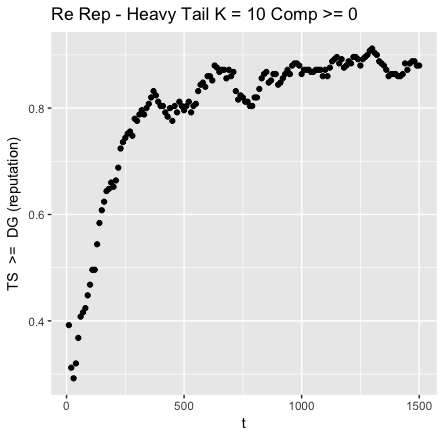
\includegraphics[scale=0.3]{figures/ts_dg_heavy_fine}
\caption*{TODO: Reduce the range of the x-axis of this so that you can understand when TS starts to do better than DG}
\end{figure}

[IDEA: take a look at the distribution of reputation induced by each algorithm under each prior]

Tables \ref{hm_nih} and \ref{hm_ht} display the results. Under Heavy Tail we see that for small warm start of $k = 20$, $DG$ gives the firm more of the market than $TS$ and $DEG$. As we increase the warm start to $k = 100, 200$ we observe that $TS$ does better than $DG$ and $DEG$. Note that, in particular for the simulations involving $TS$, the effective end of game had a median of 0. This means that the result of the simulation was \textit{completely determined by the warm start period}. Thus, when reasoning about what algorithm would win in the competition game under the HardMax decision rule we need to think about the performance of the algorithm on $k$ samples instead of $T$ samples, which may be small. For low warm start, it is thus not necessarily the case that $TS$ is the best algorithm. However, we see that under the Needle In Haystack prior $TS$ is always the best algorithm across all warm start values.

[Missing here is a discussion of the fact that with HardMax the market gets taken by one firm completely (in most simulations) as well as why this is the case.]

First, we note that the relative reputation plots were better at predicting the result of the competition game than the ``absolute" mean reputation plots. For the Needle In Haystack prior, both plots showed that $TS > DEG > DG$ in isolation and this is also the result of the competition game. However, for the Heavy Tail prior, we see that $DG, DEG > TS$ for low warm start and that, in general, $DEG > DG$ \footnote{The result that $DEG > DG$ for this prior is robust across decision rules as well.}. While the ``absolute" reputation plots imply that $TS > DEG > DG$, we see that the relative reputation plot in Figure \ref{relative_rep} implies that $DEG > DG$ and in Figure \ref{rel_rep_ht_fine} we can see that in the early rounds, $DG$ does relatively better than $TS$ and that, around $t = 100$, $TS$ does relatively better than $DG$. Note that since the median effective end of game is $0$ in \ref{hm_ht} and the agents are using the $HardMax$ decision rule, this means that the relative reputation between the two firms after $k$ samples ends up determining who takes the market in the simulations and this is precisely what the relative reputation plots tell us. Thus, looking at the relative reputation plot at time $k$ gives us a good predictor of which algorithm will take more of the market in the competition game.

Why is it that we see that $TS$ always wins under Needle in Haystack but, for lower warm start, $DG > TS$? We know that for a sufficiently long time horizon, $TS$ leads to a higher reputation than $DG$. However, in our model, firms need to incentivize the agents to select them over their competition. One possible intuition for the results here are that, in the early rounds, $TS$ engages in purposeful exploration whereas $DG$ is myopic. A consequence of exploration in our model is that it may lead to a reputational cost relative to the greedy algorithm since the sub-optimal arms pulled during exploration can harm reputation relative to the greedy algorithm. $TS$ thus incurs a relative reputational cost in the early rounds, but once it has explored enough and gained enough information it is able to recover the relative reputational loss and acquire a larger reputation than the greedy algorithm. A sufficiently large warm start allows $TS$ to explore in the early rounds and recover the reputational loss and thus win the competition game whereas a low warm start is not sufficient for this and thus $DG$ beats $TS$. Why do we only see this on Heavy Tail and not Needle in Haystack? One possible explanation for this is that learning on Heavy Tail is harder (use learning hardness metric here) and learning on Needle In Haystack is easier and thus TS needs more samples in the Heavy Tail instances compared to the Needle In Haystack instances in order to be able to recover the relative reputation loss [TODO: Explain this a bit more and with more formality. Can we have some experimental results that ``prove" this or generalize it?]

[TODO: Can we say anything general about this using the ``learning hardness" metric that we have started looking at?]

\section{Incumbent Experiment}
\label{S:7}

We now fix the same parameters as before, fixing a warm start of $k = 20$ [we should re-run this] but let $X = 200$ so that firm 2 has an ``incumbency" advantage. Recall that $X$ controls the number of rounds the firm is in the market by itself before the other firm enters and so in these rounds agents arrive and must choose firm 2. Importantly, we treat $X$ as an exogenous parameter (and not something optimally chosen by the entrant) and study the consequences of a fixed value of $X$. Thus, firm 2 is a monopolist for $X$ periods and, after $X$ rounds, firm 1 enters the market and each agent that enters in subsequent periods must select between the two firms. We want to understand what algorithms the incumbent (and the entrant) are incentivized to play. In particular, we are interested if introducing this asymmetry in entry induces firms who were previously incentivized to play $DG$ to play $TS$. As a result, we present the results of this experiment for $k = 20$ and on the Heavy Tail prior, where we saw that $DG$ was preferred to $TS$.

\begin{table}[ht]
\label{ht_incum}
\centering
\caption{Incumbent Experiment for Heavy Tail}
\begin{tabular}{rlll}
\multicolumn{3}{c}{Incumbent Algorithm} \\
\multirow{3}{*}{\rotatebox{90}{Entrant Algorithm}} \\
\hline
 & TS & DEG &  DG \\ 
 \hline
TS & \makecell{\textbf{ 0.0067 } $\pm$ 0.0092 \\Variance: 0.007 \\ ES: 100 \%} & \makecell{\textbf{ 0.023 } $\pm$ 0.017 \\Variance: 0.02 \\ ES: 99 \%} & \makecell{\textbf{ 0.064 } $\pm$ 0.027 \\Variance: 0.05 \\ ES: 97 \%} \\ 
\hline
  DEG & \makecell{\textbf{ 0.024 } $\pm$ 0.015 \\Variance: 0.02 \\ ES: 98 \%} & \makecell{\textbf{ 0.13 } $\pm$ 0.034 \\Variance: 0.09 \\ ES: 86 \%} & \makecell{\textbf{ 0.14 } $\pm$ 0.036 \\Variance: 0.1 \\ ES: 89 \%} \\ 
\hline   
   DG & \makecell{\textbf{ 0.063 } $\pm$ 0.024 \\Variance: 0.04 \\ ES: 93 \%} & \makecell{\textbf{ 0.19 } $\pm$ 0.041 \\Variance: 0.1 \\ ES: 91 \%} & \makecell{\textbf{ 0.15 } $\pm$ 0.032 \\Variance: 0.08 \\ ES: 77 \%} \\ 
\end{tabular}
\caption*{\tiny{TODO: fix table names and general table alignment. The first line in each cell contains the average market share for the entrant over $N=250$ simulations as well as a 95\% confidence interval. The second line contains the sample variance of the observed market shares and the third line contains the fraction of simulations that ended up with one principal getting $> 90\%$ of the market. Note that smaller values in the table are better for the incumbent. Market shares are calculated as the fraction of users selecting a particular firm \textit{after} the entrant has already entered (i.e. the free rounds to firm 2 do not count towards the share)}}
\end{table}

Table \ref{ht_incum} shows the results of the simulations. We observe that, for the incumbent, $TS$ is a dominant strategy. In the appendix we include additional simulations where $X = 50$ and observe that $TS$ is not always a dominant strategy in this case. Qualitatively, these results are robust across the different priors we considered as well as across agent response models. Namely, for sufficiently large $X$, $TS$ is a dominant strategy for the incumbent.

Why do we observe this reversal? The intuition for this is that competition forces the firms to worry about their reputation which dissuades them from committing to algorithms that involve pure exploration in the early rounds. This intuition is very similar to that observed in the previous section by increasing warm start. In some sense one can view allowing one firm to temporarily be a monopolist as temporarily relaxing the ``incentive" component of exploration, exploitation, and incentives so that the incumbent firm only faces the classic tradeoff between exploration and exploitation. The incumbent only needs to worry about her reputation after $X$ periods when the entrant comes into the market and again needs to worry about incentivizing agents to select them over their competition. As a result, the incumbent is incentivized to commit to an algorithm that does exploration in the early rounds since she no longer suffers the same relative reputational cost that she would suffer under competition as long as the $X$ is sufficiently large that she can begin to recover the reputational costs of exploration. Thus, counterintuitively, by allowing one firm to be a monopoly and dominate the market, we can incentivize them to play $TS$ and thus get higher social welfare than under competition. [add some more economic intuition here]

[Include some discussion about the entrant]

\section{Data and Reputation \\ as Barriers to Entry}
\label{S:8}

As the simulation results of the incumbent experiment in Table \ref{ht_incum} and in the appendix show, the incumbent usually ends up with a substantial share of the market over the entrant. The rounds where the incumbent was a monopolist provided the incumbent with free data for learning (data advantage) as well as a chance to establish a reputational advantage over a potential entrant (reputational advantage). Which plays a bigger role in preventing the entrant from being able to establish market share? We run two additional experiments, modifying the previous incumbent experiment so that in one set of simulations the reputation of the incumbent is artificially erased and another in which the information gained by the incumbent is artificially erased so that the posterior is reset to the prior.

\begin{table}[ht]
\centering
\caption{Reputation Erased Experiment} 
\begin{tabular}{rlll}
  \hline
 & TS & DEG &  DG \\ 
  \hline
TS & \makecell{ \textbf{ 0.18 } $\pm$ 0.042 \\Var:  0.1 \\ ES: 97 \% } & \makecell{ \textbf{ 0.17 } $\pm$ 0.042 \\Var:  0.1 \\ ES: 98 \% } & \makecell{ \textbf{ 0.23 } $\pm$ 0.047 \\Var:  0.2 \\ ES: 98 \% } \\ 
  DEG & \makecell{ \textbf{ 0.23 } $\pm$ 0.045 \\Var:  0.2 \\ ES: 92 \% } & \makecell{ \textbf{ 0.32 } $\pm$ 0.049 \\Var:  0.2 \\ ES: 86 \% } & \makecell{ \textbf{ 0.25 } $\pm$ 0.046 \\Var:  0.2 \\ ES: 90 \% } \\ 
   DG & \makecell{ \textbf{ 0.28 } $\pm$ 0.047 \\Var:  0.2 \\ ES: 87 \% } & \makecell{ \textbf{ 0.33 } $\pm$ 0.051 \\Var:  0.2 \\ ES: 91 \% } & \makecell{ \textbf{ 0.3 } $\pm$ 0.047 \\Var:  0.2 \\ ES: 83 \% } \\ 
   \hline
   \label{rep_erase}
\end{tabular}
\end{table}
% latex table generated in R 3.4.0 by xtable 1.8-2 package
% Sun Jul 22 14:23:06 2018
\begin{table}[ht]
\centering
\caption{Information Erased Experiment} 
\begin{tabular}{rlll}
  \hline
 & TS & DEG &  DG \\ 
  \hline
TS & \makecell{ \textbf{ 0.059 } $\pm$ 0.025 \\Var:  0.05 \\ ES: 97 \% } & \makecell{ \textbf{ 0.11 } $\pm$ 0.033 \\Var:  0.09 \\ ES: 94 \% } & \makecell{ \textbf{ 0.15 } $\pm$ 0.038 \\Var:  0.1 \\ ES: 92 \% } \\ 
  DEG & \makecell{ \textbf{ 0.11 } $\pm$ 0.031 \\Var:  0.08 \\ ES: 89 \% } & \makecell{ \textbf{ 0.19 } $\pm$ 0.038 \\Var:  0.1 \\ ES: 82 \% } & \makecell{ \textbf{ 0.18 } $\pm$ 0.038 \\Var:  0.1 \\ ES: 82 \% } \\ 
   DG & \makecell{ \textbf{ 0.17 } $\pm$ 0.038 \\Var:  0.1 \\ ES: 87 \% } & \makecell{ \textbf{ 0.22 } $\pm$ 0.042 \\Var:  0.1 \\ ES: 82 \% } & \makecell{ \textbf{ 0.26 } $\pm$ 0.043 \\Var:  0.1 \\ ES: 77 \% } \\ 
   \hline
   \label{info_erase}
\end{tabular}
\end{table}

Tables \ref{rep_erase} and \ref{info_erase} display the results of these experiments. Even with the data advantage or reputation advantage alone the incumbent ends up getting a substantial portion of the market, regardless of the algorithm played. However, fixing the same algorithm played by the incumbent and the entrant, the market share for the incumbent is always higher when the incumbent retains her reputation instead of her information. The intuition for this is that the reputational advantage protects the incumbent from ``bad" decisions or bad luck on rewards that adversely affect reputation and thus, especially in the earlier rounds, agents in the earlier rounds will still choose the incumbent which will allow the incumbent to regain the information they lost. However, with reputation re-initialized the better information does not protect the incumbent from getting unlucky with her rewards. Looking at the variability in the shares in the two experiments indicates that not only does the incumbent get a smaller market share on average in the reputation erased experiment, but the variability in the shares is also higher.

Though the setup is purely experimental, it is nonetheless interesting to look at if $TS$ still remains as a dominant strategy for the incumbent. In the information erased experiment, $TS$ is still a dominant strategy while in the reputation erased experiment it is not a dominant strategy. The intuition for this is that in the reputation erased experiment, the incumbent still has the data that she accumulated during her time as a monopolist and as a result, there is less value to an algorithm that engages in pure exploration as she wants to rebuild her reputation and thus might be better off exploiting the information she has in order to rebuild reputation instead of engaging in exploration and potentially damage her reputation. However, in the information erased experiment, she has a reputational cushion that allows for exploration so that she can regain the information that she lost and thus $TS$ remains a dominant strategy.

In the appendix we include the results of the same experiment but with different agent response models. In these experiments we get that information and reputation serve as substitutes for each other

[TODO: leave this, expound on this, or throw it out?]

Thus, we see that both information and reputation advantages alone can serve as substantial barriers to entry in our model. However, under the HardMax agent response model, we see that reputation serves as more of a barrier to entry compared to information.

\section{Varying the agent response model}
\label{S:9}

Thus far we have largely presented simulation results utilizing the deterministic HardMax rule. This is a natural decision rule where agents simply use the reputation score as a strict decision-making rule. In this section we consider the implications of adding randomness to the agent rule. What are the implications on what algorithm the firms are incentivized to play? How does the distribution of market share change?

Under the HardMax decision rule, firms need to incentivize consumers to select them over their competition by having a higher reputation. First, we consider the $HardMaxWithRandom$ decision rule discussed in the Section \ref{S:3}. Similar to the result in \citet{mansour2017competing} we find that this induces firms to play the ``better" algorithm for sufficiently long time horizon (see appendix). The intuition for this is the same as before, where, even though the firm initially suffers reputation loss from exploration, eventually the firm gets sufficiently many agents that don't need to be incentivized to select the firm in order to get a higher reputation than a ``worse" algorithm. We have a similar observation for the $SoftMax$ decision rule discussed in Section \ref{S:3}.

\begin{figure}
\label{agent_variances}
\end{figure}

We see that better algorithms are incentivized when we consider random agent response rules, but there are differences in the overall market composition. As Figure \ref{agent_variances} shows, the variance of market shares across simulations varies greatly. Under $HardMax$, we see that, in a single simulation, the market is generally ``winner take all" where one firm generally gets a large share of the market and there is a high variance. Under $HardMaxWithRandom$ we see that, in a single simulation, the market is mostly taken by one firm (but to a lower extent than under $HardMax$) and there is a lower, though still high, variance. Under $SoftMax$ we see that the market variance is very low and market shares are generally close to 50/50.

\section{Conclusion}
\label{S:10}

...

\pagebreak
\bibliography{refs}

\end{document}
